\chapter{Introduction\label{cha:intro}}
%4-8 pages
\gls{Linux}

Nowadays, consumers are increasingly opting to shop online. However, with so many retailers offering products online, arguably, consumers need better solutions to help them identify the specific product they would like to purchase at the lowest possible price. Commonly, retailers categorize consumer products, according to varying schemes (e.g., based on a company-specific taxonomy) and performing classification using manual or automated means. Unfortunately, these methods are not entirely accurate. Therefore, in this master's thesis, we aim to use machine learning techniques for multiclassification of online products and map them to a taxonomy of categories. As a by-product, this would likely also help to improve the detection of product duplicates and discover complementary product recommendations [1]. 

Despite the wide variety of existing eCommerce platforms, they all share one thing in common, i.e., the need to automatically classify their product offerings into a hierarchical taxonomy. Some research has already been done in this area by Yahoo! ([1]), eBay ([2, 3, 4]), and also outside of e-Commerce (e.g., performing hierarchical classification on web content [5]). As proposed in [2,3,5], when a hierarchical taxonomy is employed as target for classification, we could vary the set of product features or the particular multiclassification algorithm, depending on the level of the tree we are classifying into. However, to the best of my knowledge, combining the previous strategy with typical machine learning classification algorithms (e.g., SVM, kNN) has not been tried using large-scale data processing engines, such as Apache Flink or Apache Spark (e.g., to shorten runtimes and reduce training times). Indeed, there is a lot of room for improvement (e.g., increasing classification accuracy, reducing analysis times, and facilitating conducting benchmarks).

One of Germany's largest price comparison platform (idealo ([6]) offers consumers varying navigation options. Users are able to browse almost 2 million products that are labeled using more than 2000 different categories. These categories are organized into a hierarchical taxonomy, where products can be compared at a glance. For example, a Coleman Tent is classified as Leisure \& Outdoors > Camping > Tent, i.e., a Coleman Tent is classified as a Tent, which is a category that belongs to Camping, and at the same time is in the Leisure \& Outdoors’ category. Designing and implementing a system that can automatically organize products into a broad set of categories accurately is a non-trivial task.
Due to the large amounts of data handled by e-Commerce platforms every day, we need a multiclassification algorithm that can run on a large-scale data analytics system, like Spark or Flink. This should enhance runtime efficiency and offer a scalable solution. 



\section{Motivation\label{sec:moti}}

Start describing the situation as it is today or as it has been during the last years. 'Over the last few years there has been a tendency... In recent years...'. The introduction should make people aware of the problem that you are trying to solve with your concept, respectively implementation. Don't start with 'In my thesis I will implement X'.

\section{Objective\label{sec:objective}}

What kind of problem do you adress? Which issues do you try to solve? What solution do you propose? What is your goal?
'This thesis describes an approach to combining X and Y... The aim of this work is to...'

\section{Scope\label{sec:scope}}

Here you should describe what you will do and also what you will not do. Explain a little more specific than in the objective section. 'I will implement X on the platforms Y and Z based on technology A and B.'

Conclude this subsection with an image describing 'the big picture'. How does your solution fit into a larger environment? You may also add another image with the overall structure of your component.

'Figure \ref{fig:intro} shows Component X as part of ...' 
\\
\begin{figure}[htb]
  \centering
  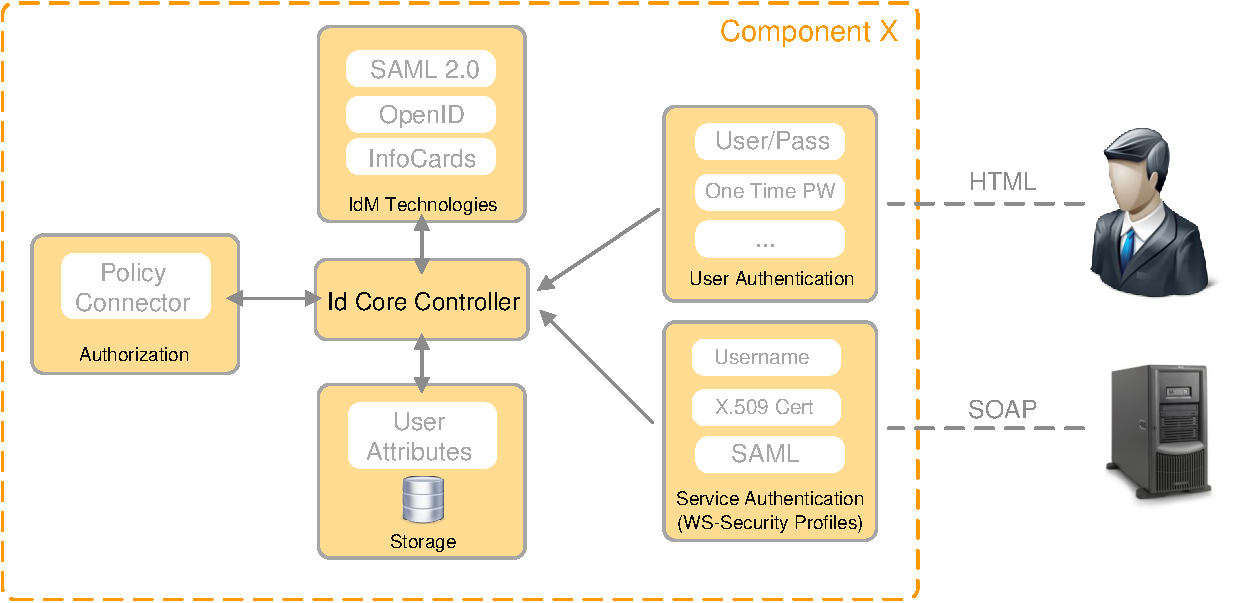
\includegraphics[width=9cm]{intro_example.pdf}\\
  \caption{Component X}\label{fig:intro}
\end{figure}

\begin{figure}[htb]
  \centering
  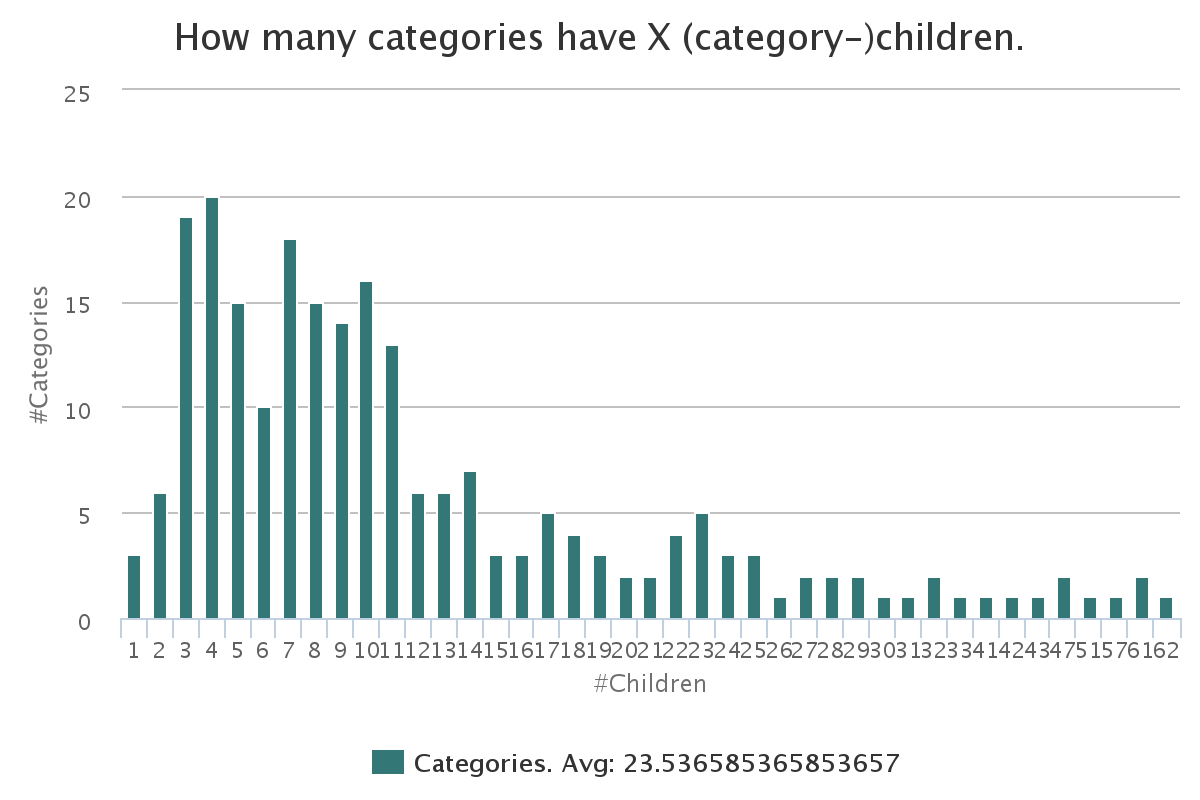
\includegraphics[width=15cm]{/plots/statistics/outdegreeCats.png}\\
  \caption{Outdegree}\label{fig:outdegree}
\end{figure}

\section{Structure\label{sec:outline}}

This Thesis is presented in X chapters:
\\
\\
\noindent This example thesis is separated into 7 chapters.
\\
\\
\textbf{Chapter \ref{cha:tf}} is usually termed 'Related Work', 'State of the Art' or 'Fundamentals'. Here you will describe relevant technologies and standards related to your topic. What did other scientists propose regarding your topic? This chapter makes about 20-30 percent of the complete thesis.
\\
\\
\textbf{Chapter \ref{cha:idealo}} analyzes the requirements for your component. This chapter will have 5-10 pages.
\\
\\
\textbf{Chapter \ref{cha:chapter4}} is usually termed 'Concept', 'Design' or 'Model'. Here you describe your approach, give a high-level description to the architectural structure and to the single components that your solution consists of. Use structured images and UML diagrams for explanation. This chapter will have a volume of 20-30 percent of your thesis.
\\
\\
\textbf{Chapter \ref{cha:chapter5}} describes the implementation part of your work. Don't explain every code detail but emphasize important aspects of your implementation. This chapter will have a volume of 15-20 percent of your thesis.
\\
\\
\textbf{Chapter \ref{cha:chapter6}} is usually termed 'Evaluation' or 'Validation'. How did you test it? In which environment? How does it scale? Measurements, tests, screenshots. This chapter will have a volume of 10-15 percent of your thesis.
\\
\\
\textbf{Chapter \ref{cha:chapter7}} summarizes the thesis, describes the problems that occurred and gives an outlook about future work. Should have about 4-6 pages.